\section{Earlier Coarse Equilibrium Adapter on PIDG}
\label{sec:pidg-rendering}
This earlier diagnostic separates appearance initialization from hard mechanical coupling; it is distinct from the dense soft-constrained hybrid above. It uses the public synthetic \emph{Balls Reaction} scene of PIDG~\cite{hong2026pidg}. It is an equilibrium reconstruction adapter, not the transient coupled-contact experiment in the main paper. It does not establish material identification from RGB, causal prediction of a new action, or quantitative accuracy at unrecorded cameras.

\paragraph{Observed inputs and physical hypotheses.}
We retain the declared 101 fitting, 11 validation and 38 test images, with supplied camera poses and a common frame-index clock. A fitting-only PIDG reconstruction initializes the radius/depth gauge. Connected color regions in the fitting images supply object-position and apparent-shape observations. Six separately represented, approximately spherical objects are an explicit initialization prior. Each object has 13 mechanical nodes, 20 tetrahedra and six localized Gaussian attachment footprints. The attachment targets are inferred position controls, not observed real grippers. The shared learned material decoder is frozen. Material descriptors are inherited from the initial image/mechanics fit and held fixed during the appearance-transfer refinement. Gravity is negligible under the unidentified physical scale, and this adapter does not solve coupled inter-object collisions.

\paragraph{Connected inference and rendering.}
For physical parameters $\eta$ and inferred boundary targets $b$, equilibrium satisfies $r(x;\eta,b)=0$. Differentiating an image loss $L$ uses
\begin{equation}
 H^\top\lambda=\frac{\partial L}{\partial x},\qquad
 \frac{dL}{d(\eta,b)}=-\lambda^\top\frac{\partial r}{\partial(\eta,b)},\quad H=\frac{\partial r}{\partial x}.
\end{equation}
The renderer therefore updates a solved physical state rather than an unconstrained deformation MLP. All 228 held-image object equilibria converge with residual below $9.73\times10^{-8}$; the minimum tetrahedral Jacobian is 0.868. These numerical checks do not establish correct contact or material identification. Gaussian centers use fixed material-coordinate bindings, covariance follows $\Sigma_t=F_t\Sigma_0F_t^\top$, and view directions are pulled into the material rotation frame for spherical-harmonic radiance. The boundary adjoint agrees with finite differences, and the binding passes affine-position and covariance tests. The earlier sparse-appearance adapter used 4,608 newly initialized Gaussians and achieved only 25.59\,dB test PSNR at $320\times180$ despite converged mechanical states. This motivates retaining fitted appearance instead of conflating its initialization error with a constitutive-model comparison.

\paragraph{Appearance-preserving reference binding.}
We transfer all 50,524 fitted Gaussian centers, full covariances, opacities and spherical-harmonic coefficients from the matched local PIDG reconstruction at the first fitting frame. At the renderer-conversion stage, RGB RMSE against the original render is $1.55\times10^{-8}$ and both renders have 56.33\,dB PSNR on that fitting image. This is a conversion check, not a test-set result. The covariance calculation matches the released rasterizer's unnormalized-quaternion convention; silently normalizing those quaternions changes the image. Material bindings use the physical state at that reference frame, including explicitly disclosed affine extrapolation outside the coarse tetrahedral mesh. Fitted appearance does not supply ground-truth hidden geometry.

\paragraph{Selection and interpretation.}
Appearance refinement and boundary refinement use only fitting RGB. Temporal controls include global pose/scale and six independently translated Gaussian boundary patches per object; joint fitting is followed by appearance-only refinement with mechanics fixed. Checkpoint selection uses validation foreground PSNR. A validation-only radiance ablation favors material-frame over world-frame directions. All candidate runs are retained. A checkpoint audit found that appearance-only regularization had changed controls behind cached geometry. Restoring the exact controls used to build that cache recovers identical live validation scores; the corrected optimizer freezes those controls explicitly. The invalid evaluation is retained in the artifact audit and excluded from the reported table. Canonical Gaussian offsets and covariance-scale corrections are bounded. PIDG is used for appearance initialization, so this is a reconstruction-assisted comparison rather than an independently initialized competitor. This released test split has also been evaluated in earlier development; it is not a newly collected confirmatory cohort. All methods are trained at $320\times180$; rendering at a larger resolution is not retraining at that resolution. The original paper's 33.31\,dB Balls Reaction score is reported under a different training setup and is not substituted for our matched baseline.

\paragraph{Measured reconstruction results.}
Table~\ref{tab:pidg-rendering} reports all 38 test images. Transferring appearance and refining boundary targets improves the connected model, while the unconstrained PIDG reconstruction remains stronger on recorded cameras. Larger output images use the same $320\times180$ training. These are held-image reconstruction scores, not forecasts of a new force.
\begin{center}
\captionof{table}{\textbf{PIDG Balls Reaction, matched image split.} Full-image / foreground PSNR (dB; higher is better), SSIM (higher) and AlexNet LPIPS (lower). The transferred model uses PIDG appearance initialization.}
\label{tab:pidg-rendering}
\begin{tabular}{llrrrr}
\toprule Output width & Method & PSNR & FG PSNR & SSIM & LPIPS \\
\midrule
320 & PIDG & 49.54 & 39.62 & 0.9987 & 0.0004 \\
320 & Ours: coarse appearance & 25.59 & 19.81 & 0.9210 & 0.0827 \\
320 & Ours: transferred appearance & 31.43 & 22.89 & 0.9710 & 0.0245 \\
\midrule
640 & PIDG & 34.48 & 25.28 & 0.9845 & 0.0086 \\
640 & Ours: coarse appearance & 25.50 & 19.28 & 0.9242 & 0.0823 \\
640 & Ours: transferred appearance & 29.86 & 20.83 & 0.9549 & 0.0442 \\
\midrule
1600 & PIDG & 31.64 & 22.41 & 0.9712 & 0.0323 \\
1600 & Ours: coarse appearance & 25.40 & 19.01 & 0.9335 & 0.0896 \\
1600 & Ours: transferred appearance & 28.68 & 19.35 & 0.9473 & 0.0662 \\
\bottomrule\end{tabular}\end{center}
\begin{center}\begin{minipage}{\textwidth}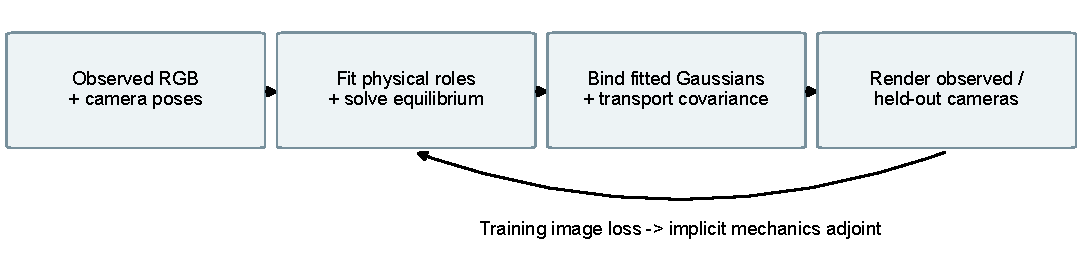
\includegraphics[width=\textwidth]{figures/pidg-rendering-loop.pdf}
\captionof{figure}{\textbf{Image loss reaches the physical state.} Boundary controls update solved equilibrium through an implicit adjoint. Appearance-only refinement then holds the selected mechanics fixed; query-time images use mechanics-transported Gaussians.}\end{minipage}\end{center}
\begin{center}\begin{minipage}{\textwidth}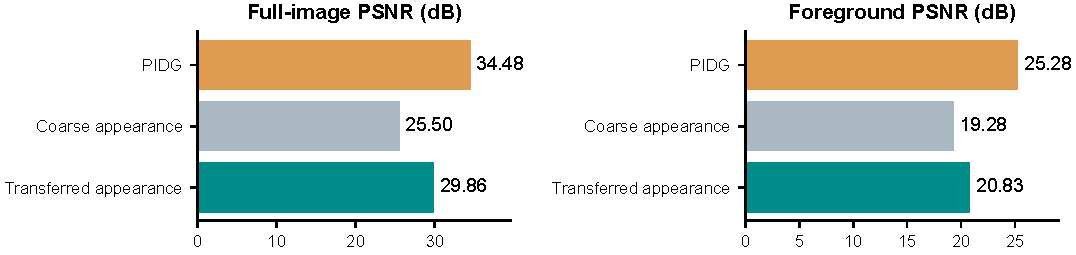
\includegraphics[width=\textwidth]{figures/pidg-rendering-metrics.pdf}
\captionof{figure}{\textbf{Aggregate recorded-camera reconstruction at width 640.} Foreground scores prevent the black background from dominating interpretation. Native PIDG remains ahead; the transferred mechanical renderer improves on its previous coarse initialization.}\end{minipage}\end{center}
\clearpage
\begin{center}\begin{minipage}{\textwidth}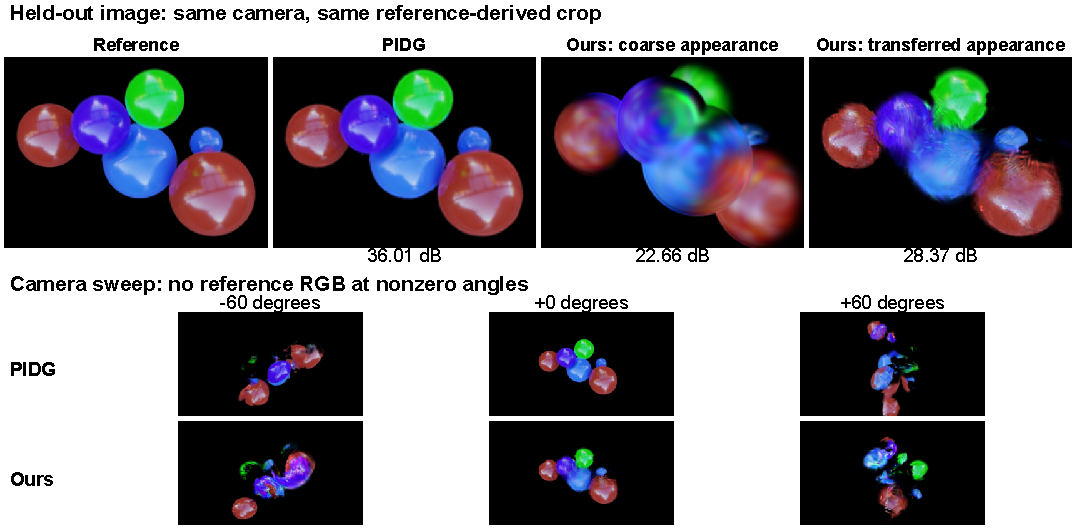
\includegraphics[width=\textwidth]{figures/pidg-rendering-comparison.pdf}
\captionof{figure}{\textbf{Appearance refinement and camera sweep.} The middle declared test time is fixed in advance. Top: identical reference-derived crop and per-frame full-image PSNR. Bottom: fixed camera offsets, with no reference RGB at nonzero angles. The spherical geometry prior contributes to coherence; these views do not prove hidden-surface accuracy or material identification.}\end{minipage}\end{center}

